\section{Experimental Results}
In this section, we first present the overall success rate for breaking the Captchas collected from the target websites. Our results shows that the overall success rates range from \textcolor{red}{45\%} to \textcolor{red}{90\%} speeding no more than 80 millseconds.
We then analyze how the success rate is affected by the number of the training Captchas.
Finally, we demonstrate the risks of our attacking approach by simulating a real world attacking process before evaluating the robustness of the secure features using variant types of text-based Captchas.

\begin{table}[t]
    \centering
    \caption{The overall success rate and average attack speeds for each Captcha scheme.}
    \label{table: overall_rate}
    \begin{tabular}{lcc}
        \toprule
        Scheme & Success rate  & Speed (ms)\\
        \midrule
        Baidu & 45\% & 70 \\
        Alipay & 86\% & 72 \\
        NetEase & 67\% & 74 \\
        VIPSHOP & 90\% & 65 \\
        TOUP & 69\% & 50 \\
        \bottomrule
    \end{tabular}
\end{table}

\begin{figure}
  \centering
  \subfigure{
    \begin{minipage}[t]{0.45\textwidth}
        
\includegraphics[width=0.15\textwidth]{fig/experiment_mnist/0-1.png}
        
\includegraphics[width=0.15\textwidth]{fig/experiment_mnist/0-2.png}
        
\includegraphics[width=0.15\textwidth]{fig/experiment_mnist/0-7.png}
        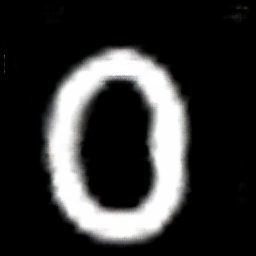
\includegraphics[width=0.15\textwidth]{fig/experiment_mnist/0-8.png}
        
\includegraphics[width=0.15\textwidth]{fig/experiment_mnist/0-9.png}
        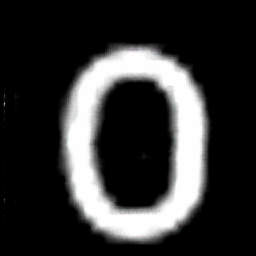
\includegraphics[width=0.15\textwidth]{fig/experiment_mnist/0-10.png}
    \end{minipage}
    }
    \subfigure{
    \begin{minipage}[t]{0.45\textwidth}
        
\includegraphics[width=0.15\textwidth]{fig/experiment_mnist/4-1.png}
        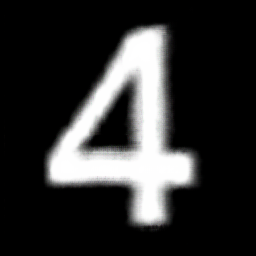
\includegraphics[width=0.15\textwidth]{fig/experiment_mnist/4-2.png}
        
\includegraphics[width=0.15\textwidth]{fig/experiment_mnist/4-5.png}
        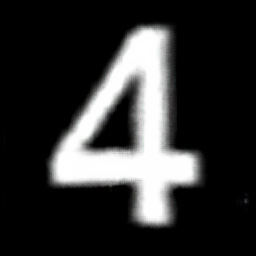
\includegraphics[width=0.15\textwidth]{fig/experiment_mnist/4-6.png}
        
\includegraphics[width=0.15\textwidth]{fig/experiment_mnist/4-7.png}
        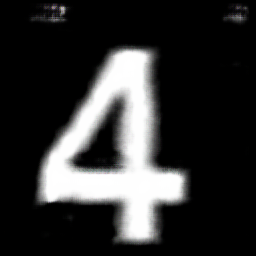
\includegraphics[width=0.15\textwidth]{fig/experiment_mnist/4-8.png}
    \end{minipage}
    }
    \subfigure{
    \begin{minipage}[t]{0.45\textwidth}
        
\includegraphics[width=0.15\textwidth]{fig/experiment_mnist/8-9.png}
        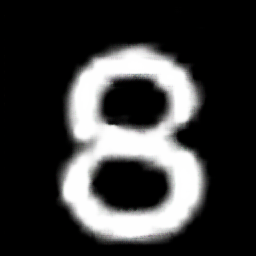
\includegraphics[width=0.15\textwidth]{fig/experiment_mnist/8-10.png}
        
\includegraphics[width=0.15\textwidth]{fig/experiment_mnist/8-3.png}
        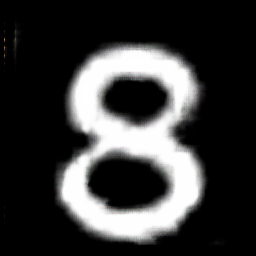
\includegraphics[width=0.15\textwidth]{fig/experiment_mnist/8-4.png}
        
\includegraphics[width=0.15\textwidth]{fig/experiment_mnist/8-5.png}
        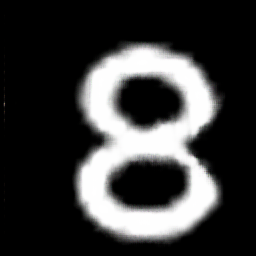
\includegraphics[width=0.15\textwidth]{fig/experiment_mnist/8-6.png} \\
        \centering (a) MNIST dataset
    \end{minipage}
    }
    \subfigure{
    \begin{minipage}[t]{0.45\textwidth}
        
\includegraphics[width=0.15\textwidth]{fig/experiment_onechar/0-1.png}
        
\includegraphics[width=0.15\textwidth]{fig/experiment_onechar/0-2.png}
        
\includegraphics[width=0.15\textwidth]{fig/experiment_onechar/0-7.png}
        
\includegraphics[width=0.15\textwidth]{fig/experiment_onechar/0-8.png}
        
\includegraphics[width=0.15\textwidth]{fig/experiment_onechar/0-9.png}
        
\includegraphics[width=0.15\textwidth]{fig/experiment_onechar/0-10.png}
    \end{minipage}
    }
    \subfigure{
    \begin{minipage}[t]{0.45\textwidth}
        
\includegraphics[width=0.15\textwidth]{fig/experiment_onechar/D-1.png}
        
\includegraphics[width=0.15\textwidth]{fig/experiment_onechar/D-2.png}
        
\includegraphics[width=0.15\textwidth]{fig/experiment_onechar/D-5.png}
        
\includegraphics[width=0.15\textwidth]{fig/experiment_onechar/D-6.png}
        
\includegraphics[width=0.15\textwidth]{fig/experiment_onechar/D-7.png}
        
\includegraphics[width=0.15\textwidth]{fig/experiment_onechar/D-8.png}
    \end{minipage}
    }
    \subfigure{
    \begin{minipage}[t]{0.45\textwidth}
        
\includegraphics[width=0.15\textwidth]{fig/experiment_onechar/o-1.png}
        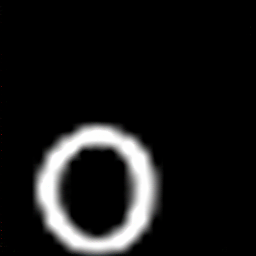
\includegraphics[width=0.15\textwidth]{fig/experiment_onechar/o-2.png}
        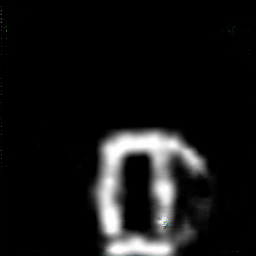
\includegraphics[width=0.15\textwidth]{fig/experiment_onechar/o-7.png}
        
\includegraphics[width=0.15\textwidth]{fig/experiment_onechar/o-8.png}
        
\includegraphics[width=0.15\textwidth]{fig/experiment_onechar/o-13.png}
        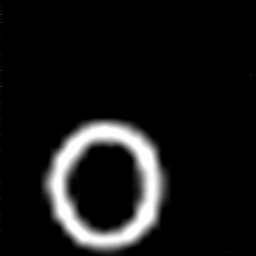
\includegraphics[width=0.15\textwidth]{fig/experiment_onechar/o-14.png} \\
        \centering (b) Single character dataset
    \end{minipage}
    }
  \caption{This figure shows some examples of original samples and their regular one transformed by our approach.}
  \label{fig: mnist_show}
\end{figure}

\subsection{Overall Success Rate}
In this experiment, the training data were synthesized used our Captcha generator, and the number of each training Captcha scheme is 20000. The corresponding testing data were collected from the target websites and its number is 2000.
\subsubsection{Evaluation using current text-based Captchas}
Table~\ref{table: overall_rate} shows the success rate for breaking different text-based Captcha schemes and it ranges from 45\% to 90\%. For VIOSHOP scheme, we are able to successfully cracking 90\% Captchas as our attacking approach can effectively remove the complex background as well as expand the space of adjacent characters. For Baidu Captchas, the success rate decreases to 45\%. This is because Baidu uses almost two different styles of Captcha scheme shown in Table~\ref{tab: captcha_show}. Further, it exploits both hollow and solid fonts. These designs make such scheme more complex than other Captchas and more difficult to be recognized.
On average, the breaking speeds for each Captcha image is no more than 80 milliseconds.
In general, our cracking success rate is far more than 1\%, the secure threshold at which the Captcha is considered ineffective~\cite{Bursztein2011Text}, which means our approach pose a great threat to current widely used text-based Captchas.

\begin{table*}[t]
    \centering
    \caption{The overall success rate and average attack speeds for each Captcha scheme.}
    \label{table: overall_rate}
    \scriptsize
    \begin{tabular}{|c|c|c|c|c|c|c|c|c|c|c|c|}
        \hline
        & \multicolumn{2}{|c|}{Success rate}& & \multicolumn{2}{|c|}{Success rate} & &\multicolumn{2}{|c|}{Success rate} & & \multicolumn{2}{|c|}{Success rate}\\
        \cline{2-3} \cline{5-6} \cline{8-9} \cline{11-12}
        \multirow{-2}{*}{Scheme} & ref.~\cite{Bursztein2011Text} & ours & \multirow{-2}{*}{Scheme} & ref.~\cite{Gao2016A} & ours & \multirow{-2}{*}{Scheme} & ref.~\cite{Bursztein2014The} & ours & \multirow{-2}{*}{Scheme} & ref.~\cite{George2017A} & ours \\
        \hline
        Authorize & 66\% & & reCaptcha & 77.2\% & 96.62\% & Baidu(2011) & 38.68\% & & reCaptcha & 66.6\% & \\
        \hline
        Blizzaer & 70\% & & Yahoo! & 5.2\% & & Baidu(2013) & 55.22\% & & Yahoo! & 57.4\% & \\
        \hline
        Captcha.net & 73\% & & Baidu & 46.6\% & 95.62\% & CNN & 51.09\% & & PayPal & 57.1\% & \\
        \hline
        Digg & 20\% & & Wikipedia & 23.8\% & 76.38\% & eBay & 51.39\% & 99.46\% & MNIST & 97.89\% & 97.45\% \\
        \hline
        eBay & 43\% & 98.9\% & QQ & 56\% & & ReCaptcha(2011) & 22.67\% & & & &\\
        \hline
        Megaupload & 93\% & & Microsoft & 16.2\% & & ReCaptcha(2013) & 22.34\% & & & & \\
        \hline
        NIH & 72\% & & Amazon & 25.8\% & 78.38\% & Wikipedia & 28.29\% & 76.38\% & & & \\
        \hline
        Reddit & 42\% & & Taobao & 23.4\% & 96.44\% & Yahoo! & 5.33\% & & & &  \\
        \hline
        Slashdot & 35\% & & Sina & 9.4\% & & & & & & & \\
        \hline
        Wikipedia & 25\% & 76.38\% & eBay & 58.8\% & 99.46\% & & & & & & \\
        \hline
    \end{tabular}
\end{table*}

\subsubsection{Evaluating using Previous text-based Captchas}
In this section, we compare our result with previous works~\cite{Bursztein2011Text,Gao2016A,Bursztein2014The} using the previous text-based Captchas.
For the previous Captchas, the real world testing data are hard to be collected because most websites have updated their Captcha scheme which is more complex than prior one. To acquire the true previous Captchas, we first use some online Captcha generator such as Captcha.net to produce the true Captcha images. We then employ the generators that previous papers has provided to generate Captchas. If neither of the two cases, we use our Captcha generator to produce the testing data.

Figure~\ref{fig: generate_show} depicts some Captcha examples of the previous real world Captchas and our generated versions that produced by our generator (Section~\ref{section: Captcha_generator}). Recall that our Captcha generator is able to generate the similar style Captchas with the real world Captcha scheme. So the generated Captcha has some subtle differences from the real one. For example, Figure~\ref{fig: generate_show} (e) shows the real Captcha deployed by Microsoft, and it slightly different from the generated one shown in (f) because the each character on Captcha image is randomly rotated and distorted.
Nevertheless, the generated Captchas contain the main features of the original real world Captchas.

\textcolor{red}{The experimental results show that}

\begin{figure}
  \centering
  \subfigure{
    \begin{minipage}[t]{0.2\textwidth}
        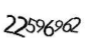
\includegraphics[width=0.9\textwidth]{fig/generate_captchas/reCAPTCHA_prior.png}\\
        \center (a) reCAPTCHA
    \end{minipage}
    }
    \subfigure{
    \begin{minipage}[t]{0.2\textwidth}
        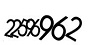
\includegraphics[width=0.9\textwidth]{fig/generate_captchas/reCAPTCHA_generator.png}\\
        \center (b) Generated version
    \end{minipage}
    }
    \subfigure{
    \begin{minipage}[t]{0.2\textwidth}
        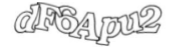
\includegraphics[width=0.9\textwidth]{fig/generate_captchas/yahoo_prior.png}\\
        \center (c) Yahoo!
    \end{minipage}
    }
    \subfigure{
    \begin{minipage}[t]{0.2\textwidth}
        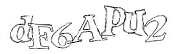
\includegraphics[width=0.9\textwidth]{fig/generate_captchas/yahoo_generator.png}\\
        \center (d) Generated version
    \end{minipage}
    }
    \subfigure{
    \begin{minipage}[t]{0.2\textwidth}
        
\includegraphics[width=0.9\textwidth]{fig/generate_captchas/microsoft_prior.png}\\
        \center (e) Microsoft
    \end{minipage}
    }
    \subfigure{
    \begin{minipage}[t]{0.2\textwidth}
        
\includegraphics[width=0.9\textwidth]{fig/generate_captchas/microsoft_generator.png}\\
        \center (f) Generated version
    \end{minipage}
    }
    \subfigure{
    \begin{minipage}[t]{0.2\textwidth}
        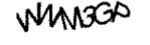
\includegraphics[width=0.9\textwidth]{fig/generate_captchas/amazon_prior.png}\\
        \center (g) Amazon
    \end{minipage}
    }
    \subfigure{
    \begin{minipage}[t]{0.2\textwidth}
        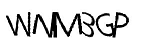
\includegraphics[width=0.9\textwidth]{fig/generate_captchas/amazon_generator.png}\\
        \center (h) Generated version
    \end{minipage}
    }
    \subfigure{
    \begin{minipage}[t]{0.2\textwidth}
        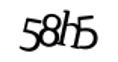
\includegraphics[width=0.9\textwidth]{fig/generate_captchas/baidu_prior.png}\\
        \center (i) Baidu
    \end{minipage}
    }
    \subfigure{
    \begin{minipage}[t]{0.2\textwidth}
        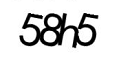
\includegraphics[width=0.9\textwidth]{fig/generate_captchas/baidu_generator.png}\\
        \center (j) Generated version
    \end{minipage}
    }
  \caption{Some examples of the real world Captchas and the corresponding generated version. The Captchas on the left column are the previous real world schemes and on the right column are the corresponding generated version.}
  \label{fig: generate_show}
\end{figure}

\begin{figure}
  \centering
  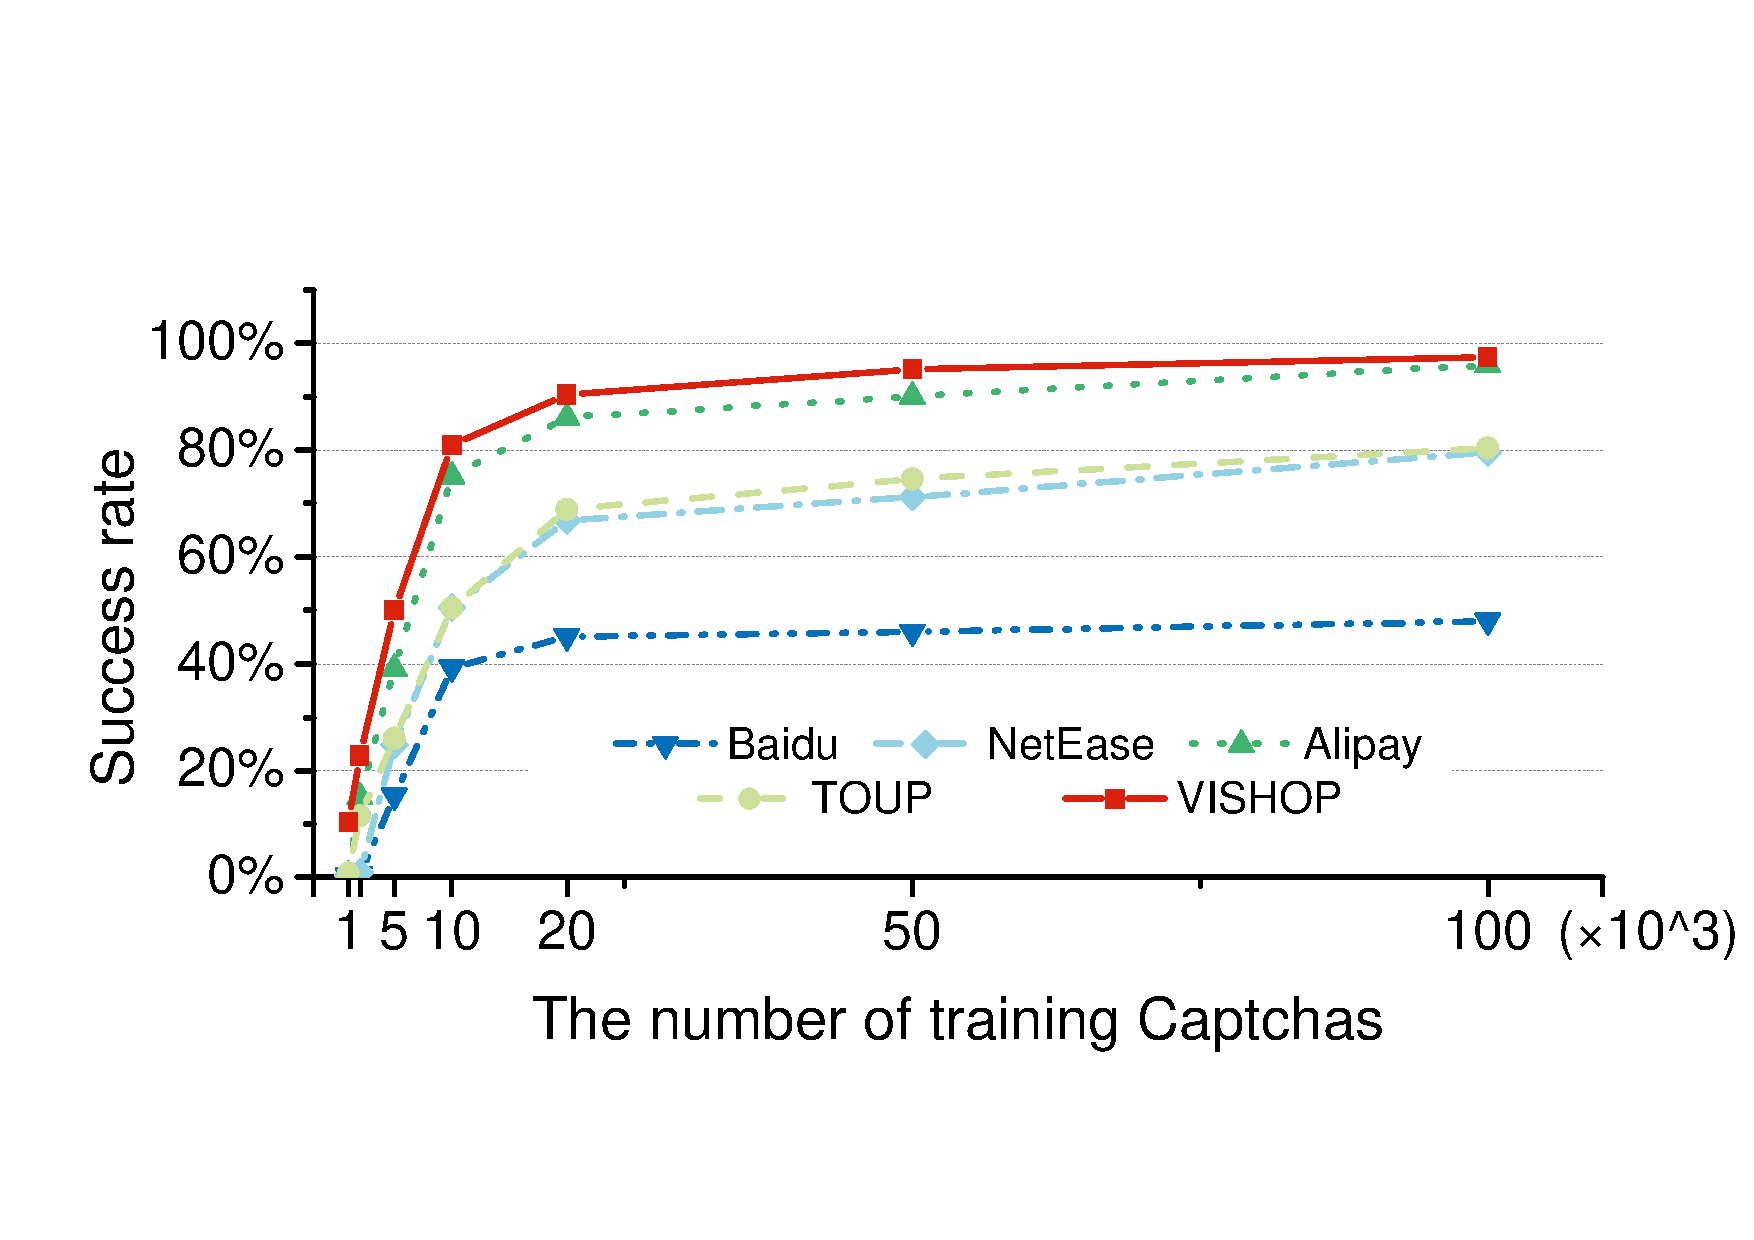
\includegraphics[width=0.45\textwidth]{fig/training_set.pdf}
  \caption{Impact of the number of training set.}
  \label{fig: training_set}
\end{figure}

\begin{table}[t]
    \centering
    \caption{Classification results on both standard MNIST and generated dataset.}
    \label{table: mnist}
    \begin{tabular}{lccc}
        \toprule
        \multicolumn{4}{c}{MNIST dataset} \\
        \midrule
        \# of per class & 100  & 200 & 500\\
        \midrule
        RCN & 97.89\% & 98.10\% & 98.60\% \\
        Ours & \textbf{91.40\%} & \textbf{94.50\%} & \textbf{98.75\%} \\
        \toprule
        \multicolumn{4}{c}{Single character dataset} \\
        \midrule
        \# of per class & 100  & 200 & 500\\
        \midrule
        RCN & 82.67\% & 81.13\% & xx.xx\% \\
        Ours & \textbf{87.68\%} & \textbf{89.84\%} & \textbf{92.29\%} \\
        \bottomrule
    \end{tabular}
\end{table}

\subsubsection{Evaluation using MNIST datasets}
We evaluate our approach using the MNIST datasets, and compared the results with the latest work~\cite{George2017A} which can recognize the MNIST with a high accuracy using a small number of training data. In this experiment, we selected 100, 200 and 500 MNIST examples for each digit for training, respectively.
Table~\ref{table: mnist} demonstrate that our approach is superior to RCN when the total number of training examples more than 5000. Indeed, RCN performs better than ours when using a small number of training data as our approach cannot correctly transformed the similar characters to the regular one.

In addition, we generated single character dataset which contains digits and English characters. Each character in this dataset is rotated and distorted. The stye of the generated dataset is a little like MNIST's style.
We use such dataset to evaluate both RCN and our approach, and the results are shown in Table~\ref{table: mnist}. It obviously show that our approach is able to recognize most characters while RCN is invalid. Figure~\ref{fig: mnist_show} shows some examples of original data and the corresponding regular version.

\subsection{Impact of the number of training data}
We would like to know how the number of training examples affects the success rate of the attack. To do so, we used all the collected Captchas and we varied the number of training Captchas from 1000 to 100000 for each scheme. Figure~\ref{fig: training_set} shows how the cracking success rate changes as the number of training Captchas increases. When the size of the training examples is 100000, our approach can break 97.5\% VISHOP Captchas, 96.6\% Alipay Captchas, 80.4\% TOUP Captchas, 79.6\% BetEase Captchas and 48\% Baidu Captchas respectively. The success rate drops significantly when the number of training Captchas is less than 10000. Beyond this point, our approach cannot extract representative features of the Captchas. The degradation features makes it difficult for our algorithm to successful recognize the content of the Captcha image.
Due to the degradation, our approach can just crack 2.65\% Baidu Captchas, 3.45\% NetEase Captchas, 4.25\% Alipay Captchas, 7.55\% TOUP Captchas and 10.4\% VISHOP Captchas respectively when the number of training examples is only 1000. Nonetheless, the success rates are higher than 1\%, the security threshold that determines whether or not the Captcha is secure.
Generally, our approach can achieve a high success rate when the number of training examples is 20000.

\begin{table*}
    \centering
    \caption{The success rate of each combinations security features}
    \label{table: combinations_resuts}
    \begin{tabular}{|c|c|c|c|c|c|c|}
        \hline
        No. & Sample Captcha & Overlapping & Rotating & Distorting & Waving & Success Rate \\
        \hline
        \tabincell{c}{1} & \tabincell{c}{
\includegraphics[width=0.1\textwidth]{fig/combination/combination1.jpg}} & \tabincell{c}{$\surd$} & \tabincell{c}{$\surd$} & & & 74.85\% \\
        \hline
        2 & \tabincell{c}{
\includegraphics[width=0.1\textwidth]{fig/combination/combination2.jpg}} & $\surd$ &  & $\surd$ & & 65.05\% \\
        \hline
        3 & \tabincell{c}{
\includegraphics[width=0.1\textwidth]{fig/combination/combination3.jpg}} & $\surd$ &  & & $\surd$ & 58.8\%  \\
        \hline
        4 & \tabincell{c}{\includegraphics[width=0.1\textwidth]{fig/combination/combination4.jpg}} &  & $\surd$ & $\surd$ & & 64.95\% \\
        \hline
        5 & \tabincell{c}{\includegraphics[width=0.1\textwidth]{fig/combination/combination5.jpg}} & & $\surd$ & & $\surd$ & 82.35\% \\
        \hline
        6 & \tabincell{c}{\includegraphics[width=0.1\textwidth]{fig/combination/combination6.jpg}} & & & $\surd$ & $\surd$ & 62.45\% \\
        \hline
        7 & \tabincell{c}{\includegraphics[width=0.1\textwidth]{fig/combination/combination7.jpg}} & $\surd$ & $\surd$ & $\surd$ & & 57.50\% \\
        \hline
        8 & \tabincell{c}{\includegraphics[width=0.1\textwidth]{fig/combination/combination8.png}} & $\surd$ & $\surd$ & $\surd$ & $\surd$ & 52.50\% \\
        \hline
        9 & \tabincell{c}{\includegraphics[width=0.1\textwidth]{fig/combination/combination9.png}} & \multicolumn{4}{|c|}{All security features} & 46.30\% \\
        \hline
    \end{tabular}
\end{table*}

\subsection{Impact of Security Features}
Intuitively, the success rate of the attack would be influenced by the number of security features used by the Captcha because the complexity of the Captcha depends on the number of the security features. To evaluate this effect, we choose the commonly used security feature such as overlapping, rotating, distortion, waving and background for the experiment.
First, we evaluate how a single commonly used security feature effect the success rate. We then evaluate our attack using our synthetic Captchas which combines of a number of commonly used security features. Note that the synthetic Captchas are more complex than current any real world Captcha scheme. At last, we generate a most complicated Captcha using all security features to evaluate our approach.

\noindent \emph{1) Evaluation of single security feature}

\textbf{Overlapping.} Overlapping decreases the space between adjacent characters and makes them collapsed, and it is considered the most effective anti-segmentation security feature~\cite{Bursztein2011Text} which is widely deployed by lots of popular websites.

We use the TOUP scheme as a case study to evaluate the security of overlapping. We modify the original TOUP Captchas through increasing character overlapping by 4, 6, 8 and 10 pixels\footnote{The overlapping of the original Captcha is no more than 3 pixels.}, respectively. For each overlapped Captchas, we generated 20000 training examples and 2000 testing examples. We then run our attack on these synthetic overlapped Captchas, and our new success rate are 65\%, 50.05\%, 42.55\% and 25.1\%, respectively.  This result demonstrates the more overlapped the characters, the less successful our approach would be. Although the success rate drops significantly when the character overlapping more than 6 pixels, it still pose a real threat to Captcha and also superior to human because human cannot recognize the Captcha when the character overlapping reaches 6 pixels~\cite{Bursztein2014The}.

\textbf{Rotating.} To evaluate how the character rotating effects the success rate, we choose the Alipay scheme for implementing the experiment as Alipay Captcha randomly rotates the character. This is more difficult than other scheme which rotates the character in one single direction. The rotating angle of Alipay is less than 15 degrees through our careful analysis. In this experiment, we increases the random rotating angle to 30 degrees. We use 20000 such Captchas for training and 2000 for testing, and our approach can achieve a success rate of 80.5\%, a little lower than the original success rate of 86.15\%. This indicates rotating does not have a positive effect in enhancing the security of Captcha under our attack.

\textbf{Distorting.} Character distortion is widely used by most current text-based Captcha schemes. It can confuse the bot program for recognizing the similar distorted characters. For example, the character "O" and the number "0" looks very similar when they are distorted. This makes the malicious bots misidentifying "O" as "0" or "0" as "O".

In this experiment, we generate 20000 training Captchas which are similar to the Alipay scheme. But the generated Captchas are more distorted than Alipay scheme. Using 2000 Captchas for testing, our approach is able to crack 67.5\% which is lower than the original success rate of 90.10\%. This indicates that although character distortion enhancing the security of Captcha to some extent, our approach can still break such Captcha with a high success rate.

\textbf{Waving.} In this evaluation, we use the Captcha generator proposed by Tuan~\emph{et al.}~\cite{Le2017Using} to produce 20000 training examples for training. Using the trained model, our approach is able to recognize 1977 out of 2000 testing Captchas, and have a success rate of 98.85\%, higher than Tuan's success rate of 93.6\%. We only failed to break 23 Captchas because our model is confused by some similar waving characters such as character "O" and number "0", character "1" and "l", \emph{etc}.  This experiment demonstrates that waving transformation of characters does not contribute to enhancing the security of Captcha under our attack.


\noindent \emph{2) Evaluation of combining security features}

Combination security features can offer a more secure protection than a single one. In this section, we perform a number of experiments to test various combinations of the security features, and evaluate how each combination effects our attack. We conduct this experiment to search whether or not having a combination can defeat against our attack. We choose four basic security features from which we design eight different combinations and we test all of them. We select Alipay Captcha for our experiments, and the size of training and test set is 20000 and 2000, respectively.

Table~\ref{table: combinations_resuts} summaries the experiment results, listing a number of combinations of security features along with its influence on the success rate of our attack.
The results suggest the following insights.  Firstly, the combinations of two or more security features are indeed more secure than just a single one. Secondly, character overlapping or distorting can offer a stronger protection than rotating or waving because overlapping or distorting changes the style of character which indeed enhances security. This can be proved by the results of experiments No. 1 - 6. Lastly, the combination of all security features has a positive effect on defeat against our attack. However, our approach is able to crack 46.30\% such Captchas, much higher than 1\% at which Captchas is considered ineffective. On the other hand, it will decreases the usability when blindly using more security features. Nonetheless, our attack still can crack all the complex schemes with a high success rate. Therefore, the text-base Captcha is no longer a secure scheme to prevent the malicious bot programs.
